\section{Implementation Plan}
The Architectural Styles and Patterns of the system to be are huge explained in Section \ref{architecturalStyle}.\\
The implementation of our system will be done module by module and component by component, most relevant and complex part of the system to be is the \textit{Controller} of the MVC model.\\
The developing of the modules must be done keeping attention in writing good \textit{Documentation of the Code}, doing \textit{Unit Test} and
finally making \textit{Code Inspection and Analysis}; these topics are explained in the Section \ref{int_test}.\\
Below there is a Figure in order to explain the implementation flow, several detailed on the \textit{Application Server} components that are the huge part of the \textit{Controller}.

\begin{figure}[H]
  \begin{center}
  	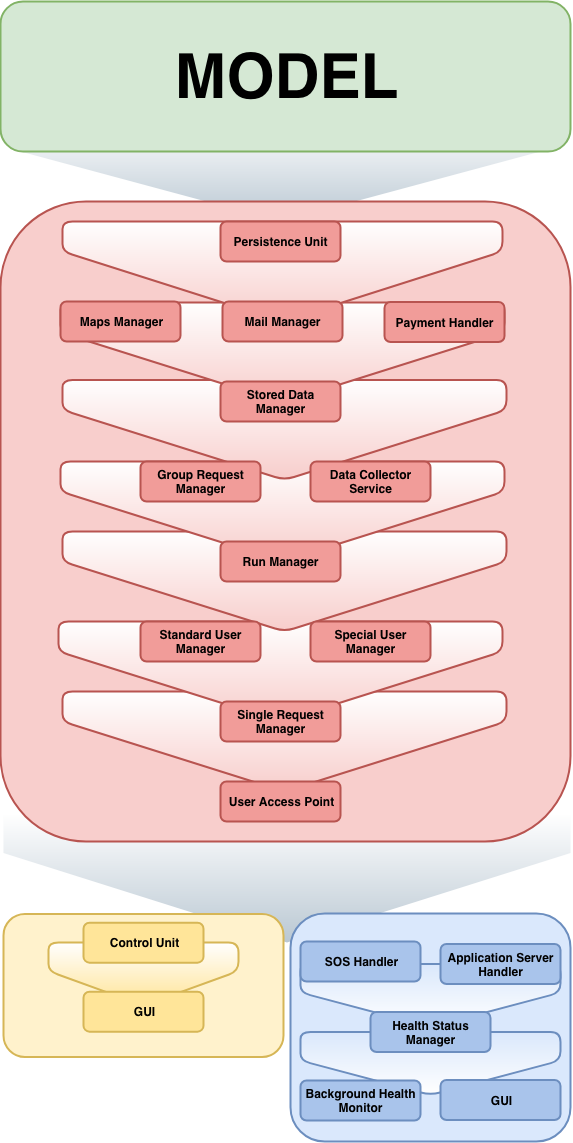
\includegraphics[height=0.59\paperheight]{./img/implementationFlow.png}
    \hspace{0.05\linewidth}
    \centering
    \caption{\textit{Implementation Plan} of the system}
		\label{img:implementationFlow}
    \end{center}
\end{figure}

\subsection{Implementation Plan Discussion}
\myparagraph{}
The \textit{Model} is the first part of the system the must be implemented. This choice is supported by the facts that the \textit{Model} is used by most of the components in the \textit{Application Server} and some part of it are represented in the \textit{Database} avoiding any type of duplication or confusion between what we consider \textit{Model} and \textit{Controller} is the main motivation of this choice.

\myparagraph{}
The second most relevant part of the system that must be developed is the \textit{Controller}, and we find in it components of the \textit{Application Server}.
\begin{itemize}
  \item \textbf{Persistence Unit} is the first component of this part that must be implemented because it manages all communication with the DBMS and communicates with a large part of the components in this part of the system.
  \item \textbf{Maps Manager}, \textbf{Mail Manger} and \textbf{Payment Handler} are components the provides the majority of services in common among other components and \textit{Maps Manager} and \textit{Payment Handler} also are the components that interfaces with the external services.
  \item \textbf{Stored Data Manager} is a critical component: it allows to manage data about users, it receives and sends data. It has an important role in data request; it provides interface for other components, for these reasons it must be developed alone.
  \item \textbf{Group Request Manager} and \textbf{Data Collector Service} provides some of the services provides by \textit{Data4Help}. They are at the base of other components so their implementation must be done keeping attention.
  \item \textbf{Run Manager} is the component that allows our system to manage the \textit{Run}'s services, fault tollerance must be guarantee. It is the core of this service and its implementation is crucial. It also provides an interface to the \textit{Standard User Manager} components and it use the \textit{Maps Manager}. component.
  \item \textbf{Standard User Manager} and \textbf{Special User Manager} are the core all actions performed by a \textit{Generic User} of \textit{Data4Help}. They communicate with most of the components described before and their implementation has to guarantee very high tolerance to fault and good performance because they represent a possible bottleneck of the application.
  \item \textbf{Single Request Manager} like some previous components it provides one of the core service of \textit{Data4Help}. Its implementation is inserted at this point because it requires some important functionalities of \textit{Standard User Manager} and \textit{Special User Manager}.
  \item \textbf{User Access Point} main function is to redirect users and their requests. It provides a way to communicate with the the internal components.
\end{itemize}

\myparagraph{}
It is the last part of the system to be that must be implemented and needs the main functionalities of the \textit{Controller}.\\
The flow of implementation of the internal components \textit{AutomatedSOS} is specified to avoid any possible problems, being a critical service.

\subsection{Implementation Choices}

\subsubsection{Database}
The choice of the \textit{Database} is MySQL 5.7 as relational DBMS and InnoDB as Database Engine. This last choice is to manage concurrency accessing same tables.

\subsubsection{Application Server}
The implementation of this important layer is the use of Java Enterprise Edition 7 (JEE) with a GlassFish Server. Java Persistence API (JPA) is used to interface with the DBMS, JAX-RS to implement RESTful APIs to interface with mobile application, \textit{Web Server} and also with the \textit{External Servicies}.

\subsubsection{Mobile App}
The mobile applications must be implemented in two different architecture respecting native languages, Swift for iOS application and Java for Android ones. The communication with the device must be done using the default frameworks of the respective system, moreover the communication with the \textit{Application Server} and \textit{External Services} must be performed with RESTful APIs.

\subsubsection{Web Server}
As we decided to implement the \textit{Application Server} with JEE, that choice is reflected to this layer. We have only to specify that the implementation of the \textit{GUI} must be performed with HTML5 and CSS; \textit{Control Unit} using JavaServer Pages (JSP).

%TODO Implementation Tree

\section{Integration and Testing}\label{int_test}
The Integration and Testing Section provides the main guidelines to explain the integration test phase, describe which tools will be used and planning integration phase in a detailed way.

\subsection{Entry Criteria}
This section describes which are the prerequisites needed before approach the integration phase. We can find three main topics the must be done before starting:
\begin{itemize}
  \item \textbf{Documentation of the Code}: Sometimes the code's documentation is understimate. Good documentation provides tools to review the code and its mean; moreover it is important in huge project, like \textit{Data4Help} one, where more people will develop the system. It makes easier the understanding of the classes functionalities and behaviour and also makes easier their reusing.\\
  Where only text documentation is not sufficient to explain a certain functionality a formal language of specification like JML (Java Modelling Language) is required
  \item \textbf{Unit Test}: All classes of the project must be tested with Unit Test that checks for each one their behaviour. Unit Test must be done using JUnit tool and line coverage of 90\% is required. Only exception of line covarge constraint must be done for the \textit{View} part of our project.
  \item \textbf{Code Inspection and Analysis}: Code Inspection and Analysis is an important phase of the testing one because with an automated tool such as SonarQube we can look for code smell possible bugs of the classes. Solving issues in this phase provides less probability of complex and big problems in the integration phase.
\end{itemize}
%Functional and non functional requirements, behaviour and purpose of the system are available in this document (\textit{DD}) and in the \textit{RASD} document.
\subsection{Elements to be Integrated}
Our system is structured in a multi-tiered client-server architecture and we can divide our system in four main layers (according to Figure \ref{img:layeredStructure}).\\
The integration of the different components in a layer must be done component by component and then when issues of internal integration will be fixed, layers integration that concerns communication between components must be performed.

\subsection{Integration Testing Strategy}
To avoid any possible of complex problems during the integration phase, like testing phase the integration phase must be performed incrementally when is possible during the growing of the system.\\
Where integration test is not possible during the developing phase, in the integration phase a bottom-up approach of integration must be follow, in order to avoid any possible of failure of the core components of the system.

\subsection{Integration Sequence}
In this Section the integration flow is explained.\\
Tables will be used to better explain the components that have a role in the integration activity.

\subsubsection{Application Server Components Integration}\label{appServCompIntRef}
Huge part of the integration component/component must be done in the \textit{Application Server} that contains a big part of the \textit{Logic} of the system. The integration must be done keeping attention and avoiding any possible issues.

\begin{center}
\begin{table}[H]
\begin{tabular}{ | l | p{0.4\textwidth} | p{0.4\textwidth} |}
  \hline
    \textbf{\#} & \textbf{Component} & \textbf{Integrated with} \\ \hline
    I01  & Stored Data Manager  & Persistence Unit \\ \hline
    I02  & Data Collector Service  & Stored Data Manager \\ \hline
    I03  & Group Request Manager  & Stored Data Manager \\ \hline
    I04  & Group Request Manager  & Payment Handler \\ \hline
    I05  & Run Manager & Persistence Unit \\ \hline
    I06  & Run Manager & Maps Manager \\ \hline
    I07  & Run Manager & Mail Manager \\ \hline
    I08  & Standard User Manager & Persistence Unit \\ \hline
    I09  & Special User Manager & Persistence Unit \\ \hline
    I10  & Standard User Manager & Mail Manager \\ \hline
    I11  & Special User Manager & Mail Manager \\ \hline
    I12  & Standard User Manager & Data Collector Service \\ \hline
    I13  & Special User Manager & Group Request Manager \\ \hline
    I14  & Standard User Manager & Run Manager \\ \hline
    I15  & Single Request Manager & Stored Data Manager \\ \hline
    I16  & Single Request Manager & Payment Handler \\ \hline
    I17  & Special User Manager & Single Request Manager \\ \hline
    I18  & Standard User Manager & Single Request Manager \\ \hline
    I19  & User Access Point & Standard User Manager \\ \hline
    I20  & User Access Point & Special User Manager \\ \hline
\end{tabular}
\caption{\textit{Application Server} components integration table}
\label{table:appServerIntegrationTable}
\end{table}
\end{center}

\begin{figure}[H]
  \begin{center}
  	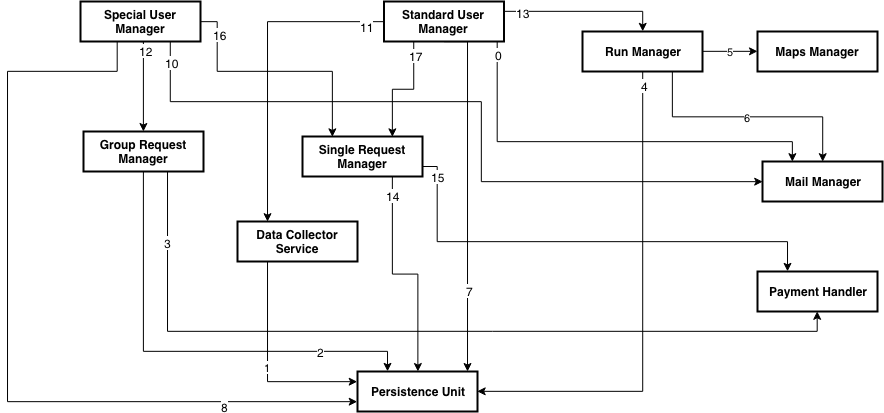
\includegraphics[width=\textwidth]{./img/appServerIntegration.png}
    \hspace{0.05\linewidth}
    \centering
    \caption{\textit{Application Server} components integration diagram}
		\label{img:appServerIntegrationDiagram}
    \end{center}
\end{figure}


\subsubsection{AutomatedSOS Components Integration}
Such as in the \textit{Application Server Components Integration} (Section \ref{appServCompIntRef}) now we want to focus our attention in the integration of \textit{AutomatedSOS} components.

\begin{center}
\begin{table}[H]
\begin{tabular}{ | l | p{0.4\textwidth} | p{0.4\textwidth} |}
  \hline
    \textbf{\#} & \textbf{Component} & \textbf{Integrated with} \\ \hline
    I01  & Health Status Manager  & Application Server Handler \\ \hline
    I02  & Background Health Monitor  & SOS Handler \\ \hline
    I03  & Background Health Monitor  & Health Status Manager \\ \hline
    I04  & GUI  & Application Server Handler \\ \hline
    I05  & GUI & Health Status Manager \\ \hline
\end{tabular}
\caption{\textit{AutomatedSOS} components integration table}
\label{table:automatedIntegrationTable}
\end{table}
\end{center}

\begin{figure}[H]
  \begin{center}
  	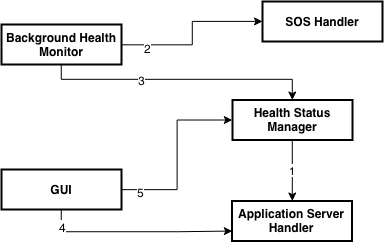
\includegraphics[width=\textwidth]{./img/automatedIntegration.png}
    \hspace{0.05\linewidth}
    \centering
    \caption{\textit{AutomatedSOS} components integration diagram}
		\label{img:automatedIntegrationDiagram}
    \end{center}
\end{figure}

\subsubsection{Subsystems Integration}
Now we present the integration sequence of subsystems. As we mentioned before a bottom-up approach must be followed.

\begin{center}
\begin{table}[H]
\begin{tabular}{ | l | p{0.28\textwidth} | p{0.28\textwidth} | p{0.28\textwidth} |}
  \hline
    \textbf{\#} & \textbf{Subsystems} & \textbf{Component} & \textbf{Integrated with} \\ \hline
    I01 & Database, Application Server & Persistence Unit & DBMS \\ \hline
    I02 & Application Server, External Servicies & Maps Handler & Maps Service \\ \hline
    I03 & Application Server, External Servicies & Payment Hendler & Payment Service \\ \hline
    I04 & Application Server, Web Server & User Access Point & Control Unit \\ \hline
    I05 & Application Server, Web Server & Run Manager & Control Unit \\ \hline
    I06 & Application Server, Mobile Client & User Access Point & Application Server Handler \\ \hline
    I07 & Application Server, Mobile Client & Run Manager & Application Server Handler \\ \hline
    I08\textsuperscript{*} & Mobile Client, External Services & SOS Handler & SOS Service \\ \hline
\end{tabular}
\caption{\textit{Subsystems integration} table.
\text{*}:this integration activity is valid only for \textit{AutomatedSOS} application}
\label{table:subsystemsIntegrationTable}
\end{table}
\end{center}
